\documentclass[12pt,a4paper]{article}

% ─── Page Layout ───────────────────────────────────────────────────────────────
\usepackage[a4paper, margin=0.8in, headheight=14pt]{geometry}

% ─── Fonts (XeLaTeX) ───────────────────────────────────────────────────────────
\usepackage{fontspec}
\usepackage{unicode-math}
\setmainfont{TeX Gyre Pagella}
\setmonofont[Scale=0.88]{TeX Gyre Cursor}
\setmathfont{Latin Modern Math}

% ─── Packages ──────────────────────────────────────────────────────────────────
\usepackage{xcolor}
\usepackage{colortbl}
\usepackage{titlesec}
\usepackage{enumitem}
\usepackage{tabularx}
\usepackage{booktabs}
\usepackage{array}
\usepackage{amsmath}
\usepackage{tikz}
\usetikzlibrary{shapes.geometric, arrows.meta, positioning, calc, fit, decorations.pathreplacing}
\usepackage{tcolorbox}
\tcbuselibrary{skins, breakable}
\usepackage{hyperref}
\usepackage{fancyhdr}
\usepackage{graphicx}
\usepackage{microtype}
\hyphenpenalty=10000
\exhyphenpenalty=10000
\sloppy
\usepackage{caption}
\usepackage{setspace}
\usepackage{multirow}
\usepackage{tocloft}

% ─── Q&A helper ────────────────────────────────────────────────────────────────
\newcommand{\Q}[1]{\textbf{#1}\par\noindent\ignorespaces}

% ─── Colour Palette ────────────────────────────────────────────────────────────
\definecolor{myred}{RGB}{196,30,58}
\definecolor{mydark}{RGB}{30,30,50}
\definecolor{mygreen}{RGB}{14,120,80}
\definecolor{myteal}{RGB}{0,130,140}
\definecolor{myamber}{RGB}{180,100,0}
\definecolor{mypurple}{RGB}{100,30,160}
\definecolor{mygray}{RGB}{246,247,249}
\definecolor{mgframe}{RGB}{180,185,200}
\definecolor{watermark}{RGB}{145,150,170}
\definecolor{hdrred}{RGB}{250,232,235}
\definecolor{hdrgreen}{RGB}{220,244,233}
\definecolor{hdrteal}{RGB}{220,242,244}
\definecolor{hdramber}{RGB}{253,242,215}
\definecolor{hdrpurple}{RGB}{238,228,255}
\definecolor{hdrgray}{RGB}{238,240,245}
\definecolor{rowalt}{RGB}{250,251,253}

% ─── Section Formatting ────────────────────────────────────────────────────────
\titleformat{\section}
  {\large\bfseries\color{myred}}{\thesection.}{0.5em}{}
  [\vspace{1pt}{\color{myred}\rule{\linewidth}{0.8pt}}]
\titleformat{\subsection}
  {\normalsize\bfseries\color{myteal}}{\thesubsection}{0.5em}{}
\titlespacing*{\section}{0pt}{18pt}{7pt}
\titlespacing*{\subsection}{0pt}{11pt}{4pt}

% ─── Paragraph ─────────────────────────────────────────────────────────────────
\setlength{\parindent}{0pt}
\setlength{\parskip}{4pt}

% ─── TOC Styling ───────────────────────────────────────────────────────────────
\renewcommand{\cfttoctitlefont}{\large\bfseries\color{myred}}
\renewcommand{\cftaftertoctitle}{\par\noindent{\color{myred}\rule{\linewidth}{0.8pt}}}
\setlength{\cftbeforetoctitleskip}{0pt}
\setlength{\cftaftertoctitleskip}{6pt}
\renewcommand{\cftsecfont}{\normalsize\bfseries\color{mydark}}
\renewcommand{\cftsecpagefont}{\normalsize\bfseries\color{mydark}}
\renewcommand{\cftsecleader}{\cftdotfill{\cftdotsep}}
\setlength{\cftbeforesecskip}{7pt}
\renewcommand{\cftsubsecfont}{\small\color{mydark}}
\renewcommand{\cftsubsecpagefont}{\small\color{mydark}}
\setlength{\cftbeforesubsecskip}{3pt}
\setlength{\cftsubsecindent}{1.4em}

% ─── Table helpers ─────────────────────────────────────────────────────────────
\renewcommand{\arraystretch}{1.45}
\setlength{\tabcolsep}{6pt}
\arrayrulecolor{mydark}
\newcolumntype{B}[1]{>{\small\bfseries\raggedright\arraybackslash}m{#1}}
\newcolumntype{Y}{>{\small\raggedright\arraybackslash}X}
\renewcommand{\tabularxcolumn}[1]{m{#1}}

% ─── Header / Footer ───────────────────────────────────────────────────────────
\pagestyle{fancy}
\fancyhf{}
\fancyhead[L]{\small\color{myred}\textbf{PE-EC701C}\;\color{mydark}--- Mobile Communication and Networks}
\fancyhead[R]{\small\color{myteal}\textbf{Module 6 Notes}}
\fancyfoot[C]{\small\color{mydark}\thepage}
\fancyfoot[R]{\small\color{watermark}\textit{\copyright\ Biraj}}
\renewcommand{\headrulewidth}{0.5pt}
\renewcommand{\footrulewidth}{0.3pt}

% ─── Hyperref ──────────────────────────────────────────────────────────────────
\hypersetup{
  colorlinks=true, linkcolor=myteal, urlcolor=myteal,
  pdfauthor={Biraj Sarkar},
  pdftitle={PE-EC701C --- Module 6 Notes}
}

% ─── tcolorbox styles ──────────────────────────────────────────────────────────
\tcbset{
  tikzbox/.style={
    colback=mygray, colframe=mgframe, boxrule=0.6pt, arc=4pt,
    left=8pt, right=8pt, top=6pt, bottom=6pt,
    colbacktitle=mgframe, coltitle=mydark,
    fonttitle=\small\bfseries
  },
  defbox/.style={
    colback=hdrgreen, colframe=mygreen, boxrule=0.8pt, arc=4pt,
    left=9pt, right=9pt, top=6pt, bottom=6pt,
    colbacktitle=mygreen, coltitle=white,
    fonttitle=\small\bfseries
  },
  formulabox/.style={
    colback=hdrteal, colframe=myteal, boxrule=0.8pt, arc=4pt,
    left=9pt, right=9pt, top=7pt, bottom=7pt,
    colbacktitle=myteal, coltitle=white,
    fonttitle=\small\bfseries
  },
  examplebox/.style={
    colback=hdramber, colframe=myamber, boxrule=0.8pt, arc=4pt,
    left=9pt, right=9pt, top=6pt, bottom=6pt,
    colbacktitle=myamber, coltitle=white,
    fonttitle=\small\bfseries
  },
  masonbox/.style={
    colback=hdrpurple, colframe=mypurple, boxrule=0.8pt, arc=4pt,
    left=9pt, right=9pt, top=6pt, bottom=6pt,
    colbacktitle=mypurple, coltitle=white,
    fonttitle=\small\bfseries
  },
  exambox/.style={
    colback=hdrpurple, colframe=mypurple, boxrule=1pt, arc=5pt,
    left=10pt, right=10pt, top=8pt, bottom=8pt,
    colbacktitle=mypurple, coltitle=white,
    fonttitle=\bfseries,
    breakable, title after break={\textbf{Frequently Asked / Viva Questions (contd.)}}}
}
\tcbset{breakable}

% ─── TikZ styles ───────────────────────────────────────────────────────────────
\tikzset{
  block/.style={rectangle, draw=myteal, fill=hdrteal,
    text width=2.4cm, align=center, minimum height=0.95cm,
    font=\small, rounded corners=3pt, line width=0.7pt},
  redblock/.style={rectangle, draw=myred, fill=hdrred,
    text width=2.4cm, align=center, minimum height=0.95cm,
    font=\small, rounded corners=3pt, line width=0.7pt},
  netnode/.style={rectangle, draw=myteal, fill=hdrteal,
    text width=1.5cm, align=center, minimum height=0.8cm,
    font=\small, rounded corners=3pt, line width=0.7pt},
  sumjunc/.style={circle, draw=myamber, fill=hdramber,
    minimum size=0.62cm, font=\small, line width=0.8pt},
  snode/.style={circle, draw=mypurple, fill=hdrpurple,
    minimum size=0.55cm, font=\footnotesize, line width=0.7pt},
  arrow/.style={-Stealth, thick, color=mydark},
  redarrow/.style={-Stealth, thick, color=myred},
  line/.style={thick, color=mydark}
}

% ═══════════════════════════════════════════════════════════════════════════════
\begin{document}
% ═══════════════════════════════════════════════════════════════════════════════

\begin{center}
  {\LARGE\bfseries\color{myred} PE-EC701C --- Mobile Communication and Networks}\\[5pt]
  {\normalsize\color{mydark} Semester VII \quad$\bullet$\quad 3L:0T:0P \quad$\bullet$\quad 3 Credits}\\[3pt]
  {\normalsize\color{myteal}\textbf{Module 6 Exam Notes: MIMO and Cellular System Examples}}\\[3pt]
  {\small\color{mydark} CGEC \;$|$\; B.Tech ECE (2023--27) \;$|$\; \textit{Biraj Sarkar}}
\end{center}
\noindent{\color{myred}\rule{\linewidth}{1.5pt}}
\vspace{2pt}

\hypersetup{linkcolor=mydark}
\tableofcontents
\hypersetup{linkcolor=myteal}
\newpage

% ===============================================================================
\section{Multiple-Input Multiple-Output (MIMO) Systems}
% ===============================================================================

MIMO systems employ multiple antennas at both the transmitter and receiver to improve link reliability and throughput without requiring extra bandwidth or transmit power.

\begin{tcolorbox}[defbox]
\textbf{MIMO System:} A wireless technology utilizing $N_T$ transmit antennas and $N_R$ receive antennas to establish a multi-antenna channel. The received signal vector $\mathbf{y}$ is modeled as:
\begin{equation}
  \mathbf{y} = \mathbf{H} \mathbf{x} + \mathbf{n}
\end{equation}
Where $\mathbf{x}$ is the $N_T \times 1$ transmitted vector, $\mathbf{y}$ is the $N_R \times 1$ received vector, $\mathbf{n}$ is the $N_R \times 1$ noise vector, and $\mathbf{H}$ is the $N_R \times N_T$ channel matrix containing complex gains $h_{ij}$ between transmit antenna $j$ and receive antenna $i$.
\end{tcolorbox}

\begin{tcolorbox}[tikzbox, title={MIMO System Model and Channel Matrix}]
\centering
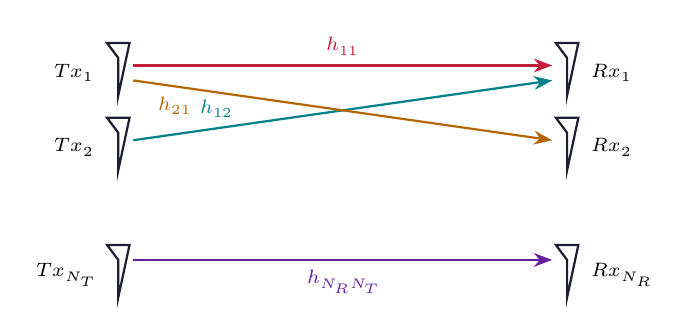
\begin{tikzpicture}[scale=0.95, every node/.style={font=\scriptsize}]
  % Tx Antennas
  \draw[line] (-2, 1.5) -- (-2, 2.0) -- (-2.15, 2.2) -- (-1.85, 2.2) -- cycle;
  \node[left] at (-2.2, 1.8) {$Tx_1$};
  
  \draw[line] (-2, 0.5) -- (-2, 1.0) -- (-2.15, 1.2) -- (-1.85, 1.2) -- cycle;
  \node[left] at (-2.2, 0.8) {$Tx_2$};
  
  \node at (-2, -0.1) {\vdots};
  
  \draw[line] (-2, -1.2) -- (-2, -0.7) -- (-2.15, -0.5) -- (-1.85, -0.5) -- cycle;
  \node[left] at (-2.2, -0.9) {$Tx_{N_T}$};

  % Rx Antennas
  \draw[line] (4, 1.5) -- (4, 2.0) -- (3.85, 2.2) -- (4.15, 2.2) -- cycle;
  \node[right] at (4.2, 1.8) {$Rx_1$};
  
  \draw[line] (4, 0.5) -- (4, 1.0) -- (3.85, 1.2) -- (4.15, 1.2) -- cycle;
  \node[right] at (4.2, 0.8) {$Rx_2$};
  
  \node at (4, -0.1) {\vdots};
  
  \draw[line] (4, -1.2) -- (4, -0.7) -- (3.85, -0.5) -- (4.15, -0.5) -- cycle;
  \node[right] at (4.2, -0.9) {$Rx_{N_R}$};

  % Channel matrix connections (sample)
  \draw[arrow, color=myred] (-1.8, 1.9) -- (3.8, 1.9) node[midway, above] {$h_{11}$};
  \draw[arrow, color=myteal] (-1.8, 0.9) -- (3.8, 1.7) node[pos=0.2, above] {$h_{12}$};
  \draw[arrow, color=myamber] (-1.8, 1.7) -- (3.8, 0.9) node[pos=0.1, below] {$h_{21}$};
  \draw[arrow, color=mypurple] (-1.8, -0.7) -- (3.8, -0.7) node[midway, below] {$h_{N_R N_T}$};
\end{tikzpicture}
\end{tcolorbox}

\subsection{Spatial Multiplexing vs. Spatial Diversity}
MIMO antennas can be used in two distinct modes to serve different system goals:
\par\noindent
{\renewcommand{\arraystretch}{1.65}%
\begin{tabularx}{\linewidth}{|B{3.2cm}|Y|Y|}
\hline
\textbf{Feature} & \textbf{Spatial Multiplexing} & \textbf{Spatial Diversity} \\
\hline
\textbf{Primary Goal} & Maximizes data rate (throughput). & Maximizes link reliability (reduces BER). \\[4pt]
\hline
\textbf{Transmission} & Transmits different data streams from each antenna simultaneously. & Transmits the same or coded data streams from multiple antennas. \\[4pt]
\hline
\textbf{Capacity Scaling} & Scales linearly with $\min(N_T, N_R)$. & No rate increase, but stabilizes signal SNR. \\[4pt]
\hline
\textbf{Key Schemes} & V-BLAST (Bell Labs Layered Space-Time). & Alamouti code, Space-Time Block Coding (STBC). \\[4pt]
\hline
\textbf{Channel Condition} & Requires high SNR and rich scattering. & Effective in poor SNR and deep fades. \\[4pt]
\hline
\end{tabularx}
}

\subsection{MIMO Channel Capacity}
If the channel state information (CSI) is known at the receiver only, and transmit power is distributed equally among all transmit antennas, the capacity is:
\begin{equation}
  C = B \log_2 \det \left( \mathbf{I}_{N_R} + \frac{\text{SNR}}{N_T} \mathbf{H} \mathbf{H}^H \right)
\end{equation}
Under independent and identically distributed (i.i.d.) Rayleigh fading, as $N_T, N_R \to \infty$, capacity scales as:
\begin{equation}
  C \approx \min(N_T, N_R) \cdot B \log_2(1 + \text{SNR})
\end{equation}

\subsection{Diversity-Multiplexing Trade-off (DMT)}
In MIMO systems, we cannot maximize both multiplexing gain and diversity gain simultaneously.
\begin{itemize}[leftmargin=*, itemsep=3pt]
  \item \textbf{Multiplexing Gain ($r$):} Measures how fast the transmission rate scales with SNR.
  \item \textbf{Diversity Gain ($d$):} Measures how fast the bit error rate (BER) decays with SNR ($P_e \propto \text{SNR}^{-d}$).
  \item \textbf{Trade-off Relation:} For a flat-fading i.i.d. MIMO channel of size $N_T \times N_R$, the optimal trade-off is a piecewise linear function. The maximum diversity gain at multiplexing gain $r$ (for integer $r$) is:
    \begin{equation}
      d^*(r) = (N_T - r)(N_R - r)
    \end{equation}
    For $r=0$ (pure diversity), $d^* = N_T N_R$. For $r=\min(N_T, N_R)$ (pure multiplexing), $d^* = 0$.
\end{itemize}

% ===============================================================================
\section{Cellular System Examples}
% ===============================================================================

\subsection{GSM (Global System for Mobile Communications)}
GSM is the definitive 2G digital cellular standard, operating primarily in the 900 MHz and 1800 MHz bands.

\begin{tcolorbox}[defbox]
\textbf{GSM Architecture:} Comprises three main subsystems:
\begin{itemize}[leftmargin=*, itemsep=2.5pt, topsep=2pt]
  \item \textbf{Mobile Station (MS):} The user handset containing the Subscriber Identity Module (SIM).
  \item \textbf{Base Station Subsystem (BSS):} Consists of the Base Transceiver Station (BTS - antennas and transceivers) and the Base Station Controller (BSC - handles radio resource allocation and handovers).
  \item \textbf{Network and Switching Subsystem (NSS):} The core network, centered on the Mobile Switching Center (MSC - routes calls) and databases: HLR (Home Location Register), VLR (Visitor Location Register), AuC (Authentication Center), and EIR (Equipment Identity Register).
\end{itemize}
\end{tcolorbox}

\begin{tcolorbox}[tikzbox, title={GSM System Architecture Block Diagram}]
\centering
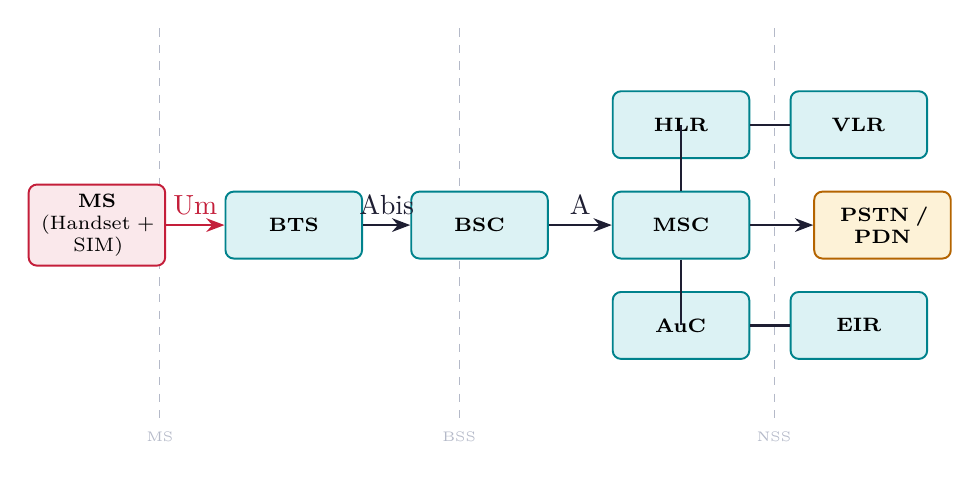
\begin{tikzpicture}[node distance=0.4cm and 0.55cm,
  sblock/.style={rectangle, draw=myteal, fill=hdrteal, text width=1.5cm,
    align=center, minimum height=0.85cm, font=\scriptsize,
    rounded corners=3pt, line width=0.7pt}]

  % Subsystems demarcation
  \draw[dashed, color=mgframe] (-2.2, 2.5) -- (-2.2, -2.5) node[below, font=\tiny] {MS};
  \draw[dashed, color=mgframe] (1.6, 2.5) -- (1.6, -2.5) node[below, font=\tiny] {BSS};
  \draw[dashed, color=mgframe] (5.6, 2.5) -- (5.6, -2.5) node[below, font=\tiny] {NSS};

  % MS Nodes
  \node[sblock, draw=myred, fill=hdrred] (ms) at (-3, 0) {\textbf{MS}\\(Handset +\\SIM)};

  % BSS Nodes
  \node[sblock] (bts) at (-0.5, 0) {\textbf{BTS}};
  \node[sblock, right=0.6cm of bts] (bsc) {\textbf{BSC}};

  % NSS Nodes
  \node[sblock, right=0.8cm of bsc] (msc) {\textbf{MSC}};
  \node[sblock, above=0.4cm of msc] (hlr) {\textbf{HLR}};
  \node[sblock, right=0.5cm of hlr] (vlr) {\textbf{VLR}};
  \node[sblock, below=0.4cm of msc] (auc) {\textbf{AuC}};
  \node[sblock, right=0.5cm of auc] (eir) {\textbf{EIR}};

  % External Network
  \node[sblock, right=0.8cm of msc, draw=myamber, fill=hdramber] (pstn) {\textbf{PSTN /}\\ \textbf{PDN}};

  % Connections
  \draw[arrow, redarrow] (ms) -- (bts) node[midway, above] {Um};
  \draw[arrow] (bts) -- (bsc) node[midway, above] {Abis};
  \draw[arrow] (bsc) -- (msc) node[midway, above] {A};
  \draw[arrow] (msc) -- (pstn);
  
  \draw[line] (msc) |- (hlr);
  \draw[line] (msc) |- (auc);
  \draw[line] (hlr) -- (vlr);
  \draw[line] (auc) -- (eir);
\end{tikzpicture}
\end{tcolorbox}

\subsubsection{GSM Channels}
GSM uses a combination of FDMA and TDMA. Each carrier is 200 kHz wide, divided into 8 time slots (users). Channels are divided into:
\begin{itemize}[leftmargin=*, itemsep=3.0pt]
  \item \textbf{Physical Channel:} A specific RF carrier frequency and time slot number.
  \item \textbf{Logical Channels:} Mapped onto physical channels to carry specific types of data.
    \begin{itemize}[leftmargin=*, itemsep=2.5pt, topsep=2pt]
      \item \textbf{Traffic Channels (TCH):} Carry digitized speech or user data.
      \item \textbf{Control Channels (CCH):} Carry signaling and control information:
        \begin{itemize}[leftmargin=*, itemsep=2pt, topsep=2pt]
          \item \textit{Broadcast Channels (BCH):} Broadcast system parameters (BCCH) and frequency correction (FCCH/SCH).
          \item \textit{Common Control Channels (CCCH):} Handle paging (PCH) and random access (RACH) to set up calls.
          \item \textit{Dedicated Control Channels (DCCH):} Handle registration and SMS.
        \end{itemize}
    \end{itemize}
\end{itemize}

\subsection{GPRS and EDGE}
\begin{itemize}[leftmargin=*, itemsep=3pt]
  \item \textbf{GPRS (General Packet Radio Service - 2.5G):} Introduces packet switching to the circuit-switched GSM core. Adds two new nodes: GGSN (Gateway GPRS Support Node) and SGSN (Serving GPRS Support Node). Supports data rates up to 115 kbps using GMSK modulation.
  \item \textbf{EDGE (Enhanced Data Rates for GSM Evolution - 2.75G):} Updates the modulation scheme from GMSK to \textbf{8-PSK} (Phase Shift Keying). Because 8-PSK maps 3 bits per symbol (instead of 1 bit in GMSK), EDGE triples the data rate of GSM/GPRS, achieving throughputs up to 384 kbps within the same 200 kHz channels.
\end{itemize}

\subsection{IS-95 (cdmaOne)}
IS-95 is the first CDMA-based 2G standard, operating in 1.25 MHz channels.
\begin{itemize}[leftmargin=*, itemsep=3pt]
  \item \textbf{Forward Link Channels (Base Station to Mobile):} Modulated using Walsh codes (length 64) for user separation and a pilot PN sequence. Channels include Pilot, Sync, Paging, and Forward Traffic Channels.
  \item \textbf{Reverse Link Channels (Mobile to Base Station):} Separated using unique offsets of a long PN code. Channels include Access and Reverse Traffic Channels.
\end{itemize}

\subsection{3G Standards: WCDMA and CDMA2000}
\begin{itemize}[leftmargin=*, itemsep=3pt]
  \item \textbf{WCDMA (Wideband CDMA / UMTS):} The dominant 3G standard. Operates in 5 MHz channels (chip rate of 3.84 Mcps). Supports asynchronous base stations and coherent detection on the uplink using pilot symbols.
  \item \textbf{CDMA2000:} A 3G standard evolution of IS-95. Uses a chip rate of 1.2288 Mcps (1xRTT) and is backward compatible with IS-95 hardware.
\end{itemize}

% ===============================================================================
% MANDATORY QUICK REVISION PAGE
% ===============================================================================
\newpage
\begin{center}
  {\large\bfseries\color{myred} Quick Revision --- Module VI}\\[3pt]
  {\small\color{mydark} MIMO and Cellular System Examples $|$ PE-EC701C}
\end{center}
\noindent{\color{myred}\rule{\linewidth}{1.2pt}}
\vspace{4pt}

\begin{tcolorbox}[formulabox, title={\textbf{Key Formulas at a Glance}}]
\renewcommand{\arraystretch}{1.3}
\begin{tabularx}{\linewidth}{B{5.5cm} X}
MIMO System Equation & $\mathbf{y} = \mathbf{H} \mathbf{x} + \mathbf{n}$ \\
MIMO Capacity (No CSIT) & $C = B \log_2 \det \left( \mathbf{I}_{N_R} + \frac{\text{SNR}}{N_T} \mathbf{H} \mathbf{H}^H \right)$ \\
MIMO Asymptotic Capacity & $C \approx \min(N_T, N_R) \cdot B \log_2(1 + \text{SNR})$ \\
Optimal DMT Trade-off & $d^*(r) = (N_T - r)(N_R - r)$ \\
GSM Carrier Bandwidth & $B = 200 \text{ kHz}$ \quad (divided into 8 time slots) \\
EDGE Modulation Update & GMSK (1 bit/symbol) $\to$ 8-PSK (3 bits/symbol) \\
IS-95 Channel Bandwidth & $B = 1.25 \text{ MHz}$ \quad (chip rate = 1.2288 Mcps) \\
WCDMA Channel Bandwidth & $B = 5.0 \text{ MHz}$ \quad (chip rate = 3.84 Mcps)
\end{tabularx}
\end{tcolorbox}

\begin{tcolorbox}[defbox, title={\textbf{One-Line Definitions}}]
\begin{itemize}[leftmargin=*, itemsep=2.5pt, topsep=0pt]
  \item \textbf{MIMO:} Using multiple antennas at transmitter and receiver to boost data rate and reliability.
  \item \textbf{Spatial Multiplexing:} Transmitting independent data streams from multiple antennas to increase throughput.
  \item \textbf{Spatial Diversity:} Sending coded redundant signals from multiple antennas to increase link reliability.
  \item \textbf{GSM BSC:} Node in BSS responsible for radio channel allocation and mobile handover management.
  \item \textbf{HLR:} Home Location Register, the central database storing subscription details and location info for home users.
  \item \textbf{GPRS SGSN:} Node responsible for packet routing, mobility management, and authentication of packet data.
  \item \textbf{8-PSK:} Modulation scheme used in EDGE mapping 3 bits per symbol, tripling GPRS data rates.
\end{itemize}
\end{tcolorbox}

\begin{tcolorbox}[exambox, title={\textbf{Frequently Asked / Viva Questions}}]
\begin{enumerate}[topsep=0pt, label=\textbf{Q\arabic*.}, itemsep=5pt]
  \item \Q{Compare spatial multiplexing and spatial diversity in MIMO systems.}
    Spatial multiplexing transmits different data streams from each antenna, maximizing data rate ($C \propto \min(N_T, N_R)$). Spatial diversity transmits redundant coded versions of the same signal, maximizing link reliability.
  \item \Q{Explain the diversity-multiplexing trade-off (DMT).}
    A MIMO channel can provide multiplexing gain $r$ and diversity gain $d$ simultaneously, but they are inversely related: $d^*(r) = (N_T - r)(N_R - r)$. You cannot maximize both at the same time.
  \item \Q{Draw and explain the GSM BSS architecture.}
    The Base Station Subsystem (BSS) contains the Base Transceiver Station (BTS) which handles the RF transmission and antennas, and the Base Station Controller (BSC) which manages handover decisions and radio channel allocations.
  \item \Q{Define the roles of HLR and VLR in GSM.}
    HLR is the master database containing subscription profiles and current location coordinates of all home subscribers. VLR is a local database containing profiles of roaming users currently inside that MSC's area.
  \item \Q{How does EDGE achieve higher data rates than GPRS within the same channel bandwidth?}
    EDGE replaces GMSK modulation (1 bit per symbol) with 8-PSK modulation (3 bits per symbol). By mapping 3 bits per symbol, it triples the data rate to 384 kbps without widening the 200 kHz channel.
  \item \Q{What are the functions of the SGSN and GGSN nodes in GPRS?}
    The Serving GPRS Support Node (SGSN) handles local packet routing and mobility management. The Gateway GPRS Support Node (GGSN) acts as the router and interface between the cellular network and external packet data networks (Internet).
  \item \Q{Describe the forward link channel structure of the IS-95 CDMA standard.}
    It uses a 1.25 MHz channel. Signals are separated using 64-length orthogonal Walsh codes. Channels include a Pilot channel, Sync channel, Paging channel, and Forward Traffic channels.
  \item \Q{What is WCDMA? State its chip rate and channel bandwidth.}
    WCDMA is a wideband 3G standard. It operates in 5 MHz channels with a chip rate of 3.84 Mcps, enabling high-rate packet data and asynchronous base stations.
  \item \Q{Define physical and logical channels in GSM.}
    A physical channel is a specific combination of RF carrier frequency and time slot number. A logical channel is a category of data (e.g., speech or paging control) mapped onto the physical time slot.
  \item \Q{Explain how the capacity of a MIMO link scales as the antenna arrays grow.}
    If the channel exhibits rich scattering and CSI is known at the receiver, the capacity scales linearly with the minimum number of transmit and receive antennas: $C \propto \min(N_T, N_R)$.
  \item \Q{What is V-BLAST and how does it relate to MIMO?}
    Vertical Bell Laboratories Layered Space-Time (V-BLAST) is a spatial multiplexing transmitter architecture that demultiplexes a high-speed data stream into parallel sub-streams without coding across antennas.
  \item \Q{Why does IS-95 CDMA require a pilot channel on the forward link?}
    The pilot channel transmits a continuous, unmodulated PN sequence. The mobile station uses it to establish phase and timing references, enabling coherent demodulation of traffic channels.
\end{enumerate}
\tcbset{colbacktitle=myteal, coltitle=white}
\end{tcolorbox}

\begin{tcolorbox}[tikzbox, title={Comparison of 2G, 2.5G, 2.75G, and 3G Systems}]
\renewcommand{\arraystretch}{1.4}
\par\noindent
{\renewcommand{\arraystretch}{1.55}%
\begin{tabularx}{\linewidth}{|B{2.8cm}|Y|Y|Y|Y|}
\hline
\textbf{Feature} & \textbf{GSM (2G)} & \textbf{GPRS (2.5G)} & \textbf{EDGE (2.75G)} & \textbf{WCDMA (3G)} \\[4pt]
\hline
\textbf{Switch Type} & Circuit. & Packet + Circuit. & Packet + Circuit. & Packet + Circuit. \\
\hline
\textbf{Modulation} & GMSK. & GMSK. & 8-PSK. & QPSK. \\
\hline
\textbf{Max Rate} & 9.6 kbps. & 115 kbps. & 384 kbps. & 2 Mbps. \\
\hline
\textbf{Bandwidth} & 200 kHz. & 200 kHz. & 200 kHz. & 5.0 MHz. \\
\hline
\end{tabularx}
}
\tcbset{colbacktitle=myteal, coltitle=white}
\end{tcolorbox}

\end{document}
